The result of the implementation is described in the following demonstration case, where the goal is to build a lego figure, called ``Space Pirate'', seen in Figure~\ref{demoCaseGoal}. The walkthrough will cover both the Google Glass version as well as the smartphone version. The Lego parts will already be partially assembled in order to reduce the number of slides, as the general idea of the application will still be presented. There are four different components used to construct the Space Pirate. All of the components can be seen in Figure~\ref{demoCaseRaw}.

	\begin{figure}[H]%ht!]
		\centering
		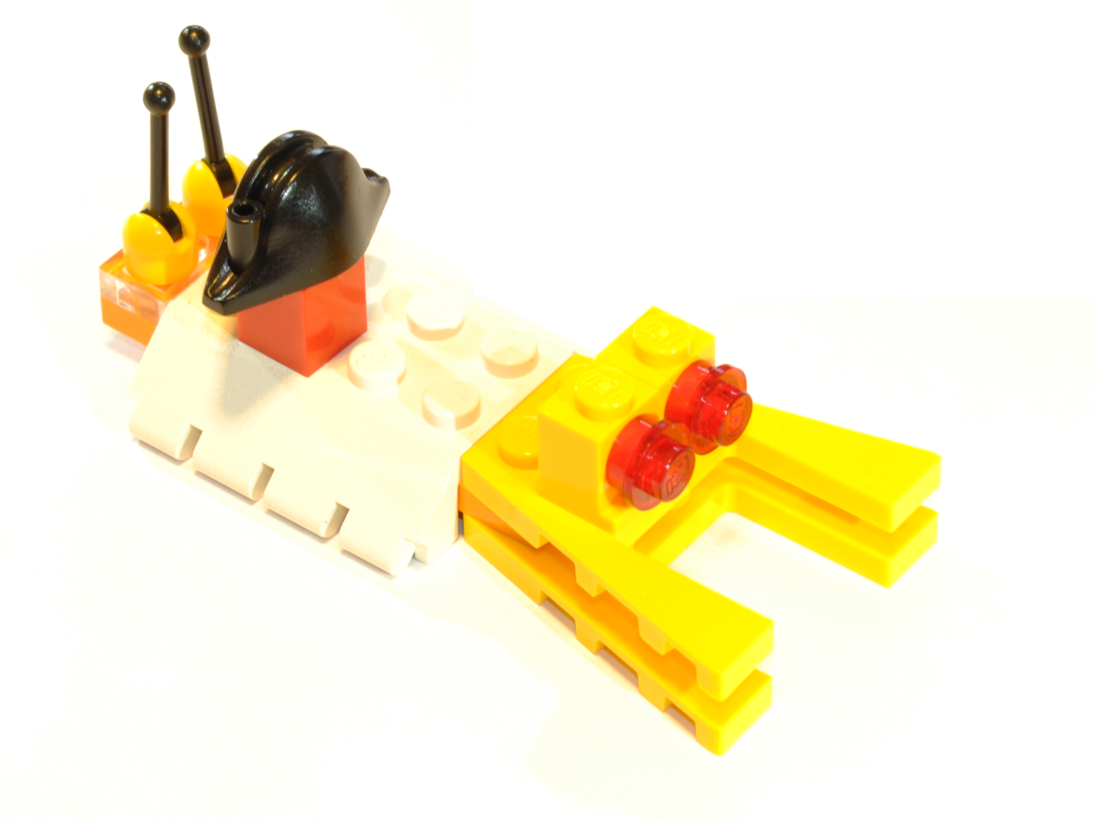
\includegraphics[width=90mm]{images/rawImages/BILD_6}
		\caption{Space Pirate.}
		\label{demoCaseGoal}
	\end{figure}

	\begin{figure}[H]%ht!]
		\centering
		\subfloat[Steering.]{{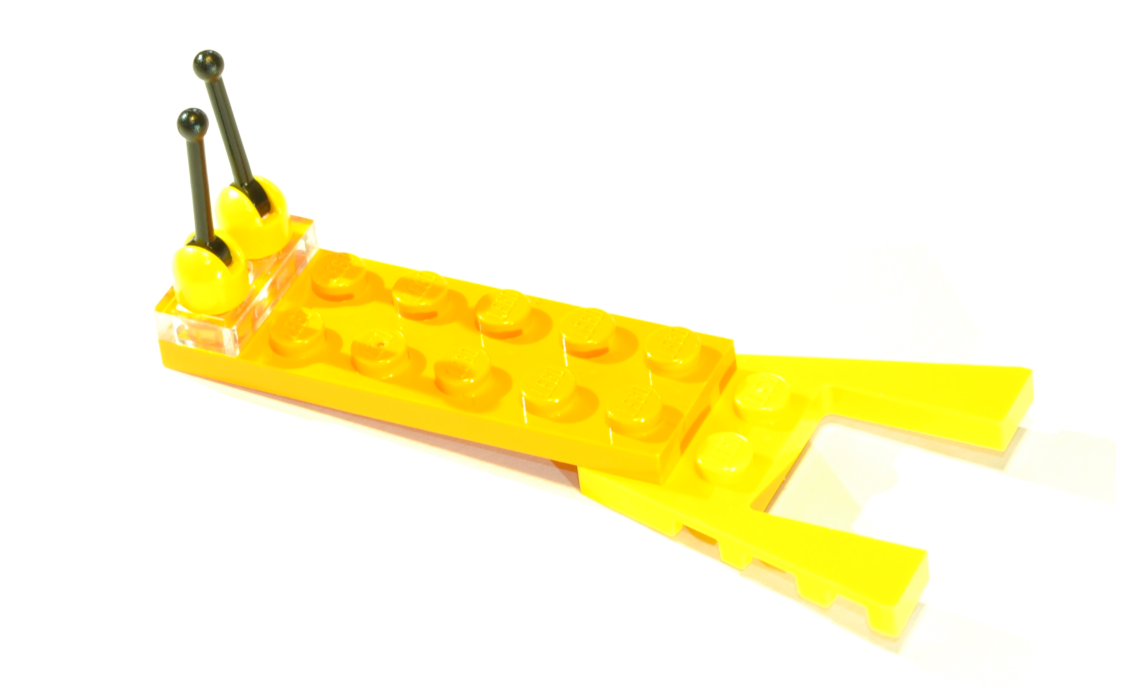
\includegraphics[width=50mm]{images/rawImages/BILD_1}}}
		\qquad
		\subfloat[Tail Light.]{{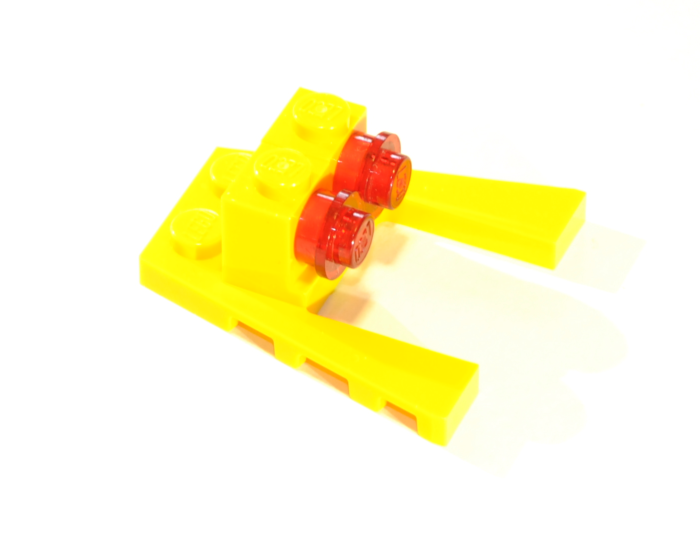
\includegraphics[width=50mm]{images/rawImages/BILD_2}}}
		\qquad
		\subfloat[Body.]{{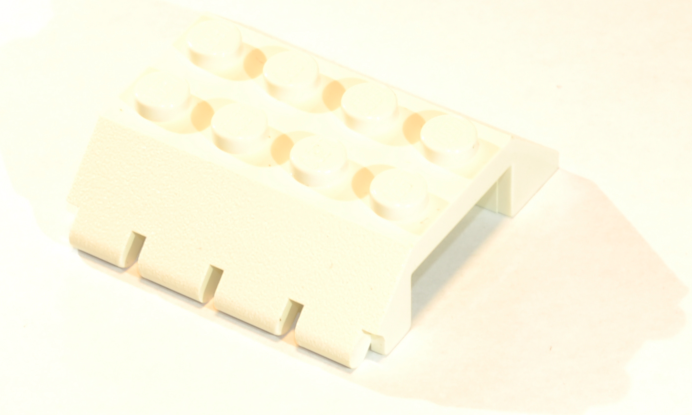
\includegraphics[width=50mm]{images/rawImages/BILD_3}}}
		\qquad
    		\subfloat[Pirate.]{{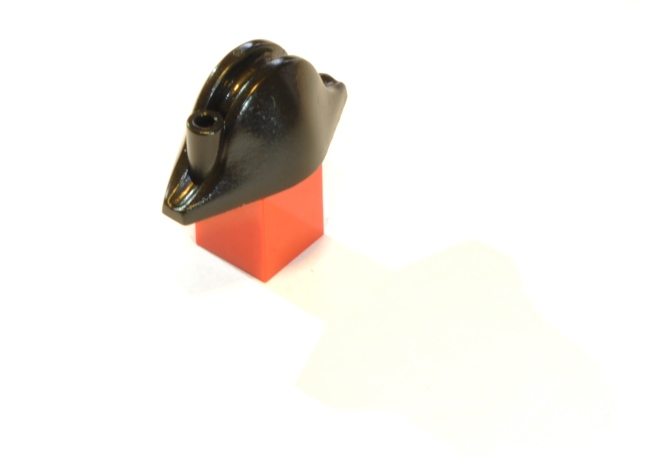
\includegraphics[width=50mm]{images/rawImages/BILD_4}}}
		\qquad
		\caption{Components.}
		\label{demoCaseRaw}
	\end{figure}

In order to receive any information on the product the user must scan the product specific QR code, as seen in Figure~\ref{demoCaseQRLoad}~(a) and in Figure~\ref{demoCaseQRLoad}~(c). When the QR code has been scanned the information will be downloaded, as seen in Figure~\ref{demoCaseQRLoad}~(b) and in Figure~\ref{demoCaseQRLoad}~(d).

	\begin{figure}[ht!]
		\centering
		\subfloat[Scanning a QR code in the Google Glass application.]{{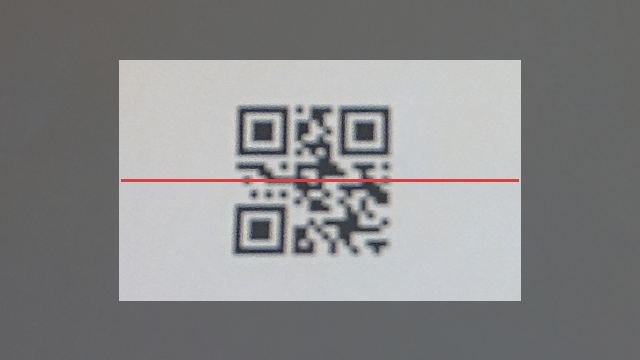
\includegraphics[width=60mm]{images/demo/qrCodeNew}}}
		\qquad
		\subfloat[Loading in the Google Glass application.]{{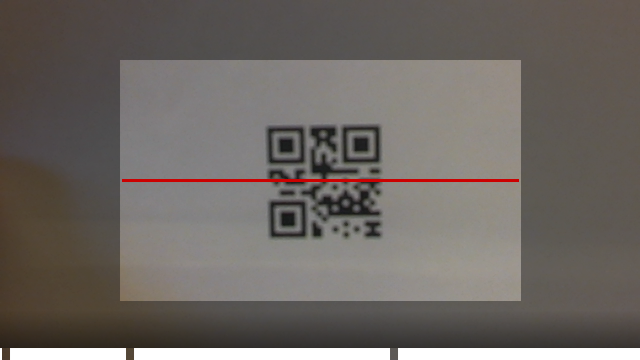
\includegraphics[width=60mm]{images/demo/loadingBar}}}
		\qquad
		\subfloat[Scanning a QR code in the smartphone application.]{{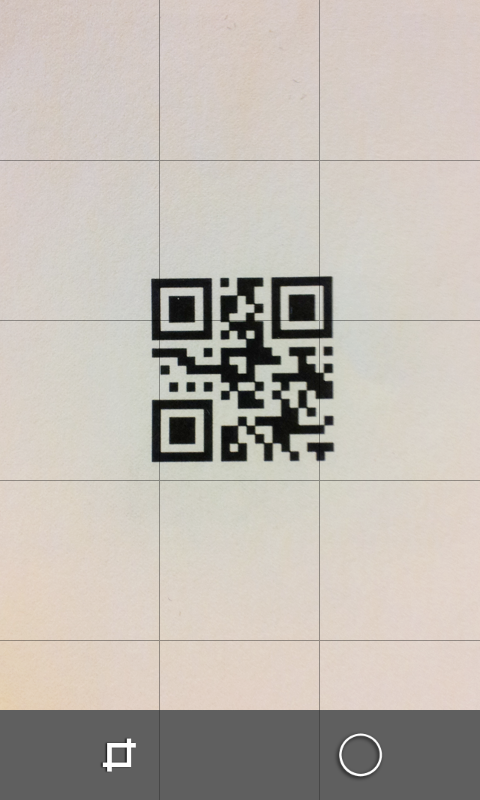
\includegraphics[width=60mm]{images/demo/smartphone/qrCodeNew}}}
		\qquad
    		\subfloat[Loading in the smartphone application.]{{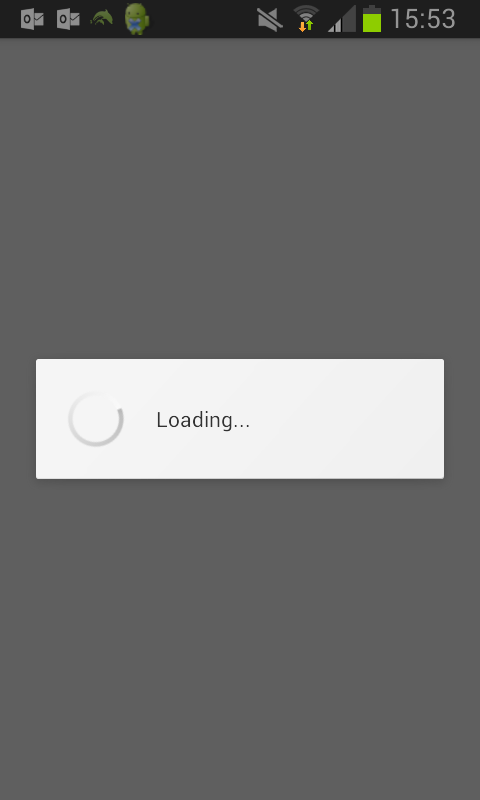
\includegraphics[width=60mm]{images/demo/smartphone/loadingSpinner}}}
		\qquad
		\caption{Scanning and loading screens.}
		\label{demoCaseQRLoad}
	\end{figure}

The first slide the user sees, when the product information has been downloaded and is displayed to the user, is the title slide. The title slide for the Space Pirate can be seen Figure~\ref{demoCase1} and shows the name of the product, as well as an image of what the product will look like when constructed. In Figure~\ref{demoCase1}~(a) the Google Glass application can be seen, and in Figure~\ref{demoCase1}~(b) the smartphone application can be seen. Using the Google Glass application users can, by saying ``ok glass'', bring up the voice command menu, seen in Figure~\ref{demoCaseVoiceCommand}, and navigate through the application. In the smartphone application, no voice commands exist, but users may use the two buttons on the title slide in order to skip through the slides to either the components or the instructions. However, in both the Google Glass application and the smartphone application users can simply swipe, using a finger, to the next slide in line. 

	\begin{figure}[ht!]
		\centering
		\subfloat[The title card in the Google Glass application.]{{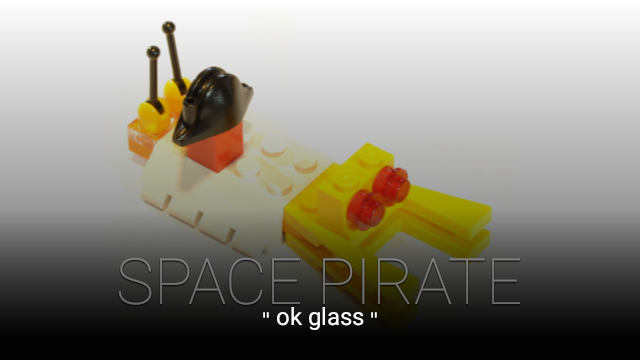
\includegraphics[width=60mm]{images/demoCase/1}}}
		\qquad
		\subfloat[The title slide in the smartphone application.]{{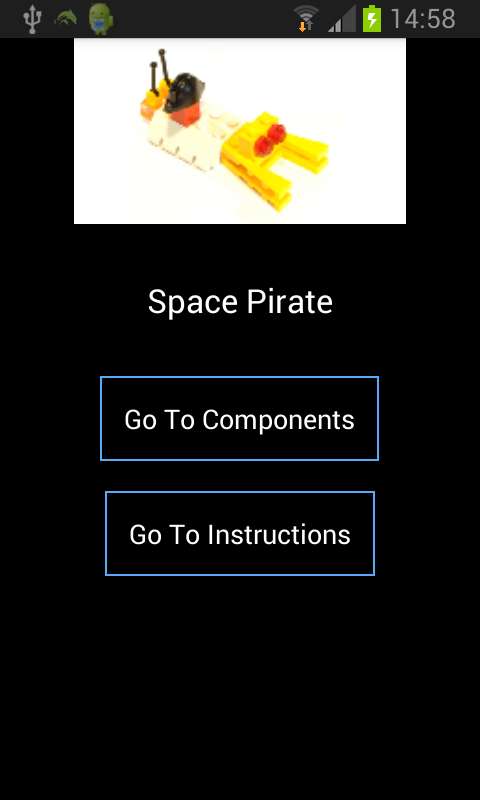
\includegraphics[width=60mm]{images/demoCase/1sp}}}
		\caption{The title slide.}
		\label{demoCase1}
	\end{figure}	

	\begin{figure}[H]%ht!]
		\centering
		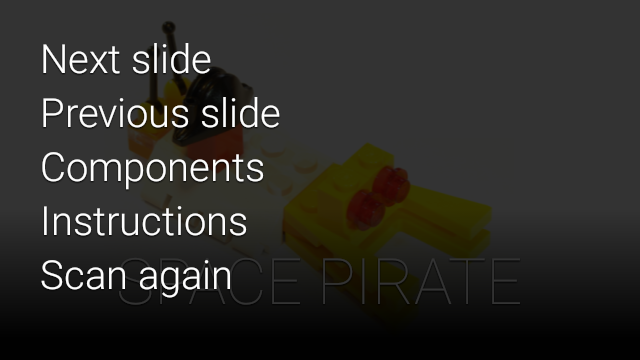
\includegraphics[width=90mm]{images/demoCase/glassVoiceCommand}
		\caption{The voice command menu.}
		\label{demoCaseVoiceCommand}
	\end{figure}


The second slide of the application is the first component slide, seen in Figure~\ref{demoCaseSteering}. Here the user sees the first component needed for constructing the Space Pirate, which is the Steering component, seen in Figure~\ref{demoCaseSteering}~(d). While the Google Glass application is fixed in its layout, the smartphone application can be altered in terms of the screen orientation. This is because while Google Glass is mounted on the user's head and may not be rotated, the smartphone can. As such the smartphone application can be viewed in either portrait orientation, seen in Figure~\ref{demoCaseSteering}~(b), or in landscape orientation, seen in Figure~\ref{demoCaseSteering}~(c). In both cases the image allocates the same percentage of screen space in width as the image does in the Google Glass application, which is \(\frac{3}{8}\). For the remainder of this demonstration walkthrough of the application the screen shots of the smartphone application will be in landscape mode, but it should be noted that all slides in the smartphone application may be viewed in both portrait orientation and landscape orientation.

	\begin{figure}[H]%ht!]
		\centering
		\subfloat[The first component card.]{{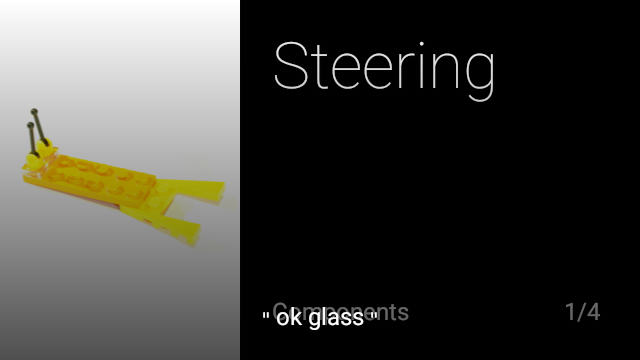
\includegraphics[width=60mm]{images/demoCase/2}}}
		\qquad
		\subfloat[The first component slide in portrait screen orientation.]{{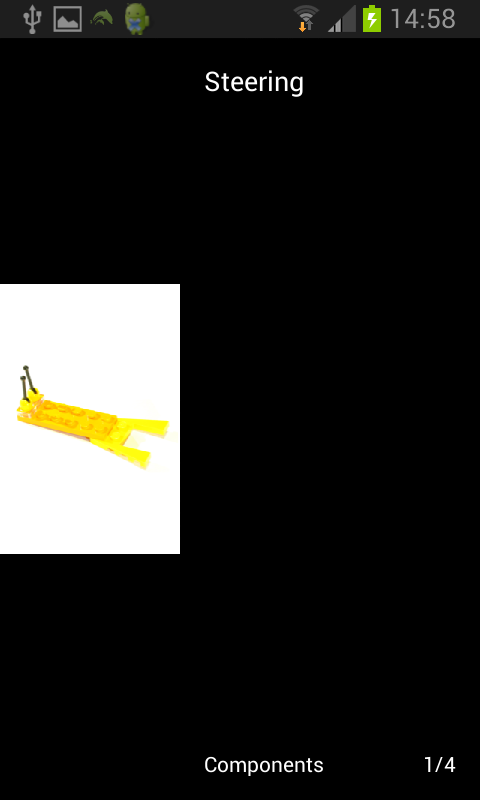
\includegraphics[width=60mm]{images/demoCase/2spP}}}
		\qquad
		\subfloat[The first component slide in landscape screen orientation.]{{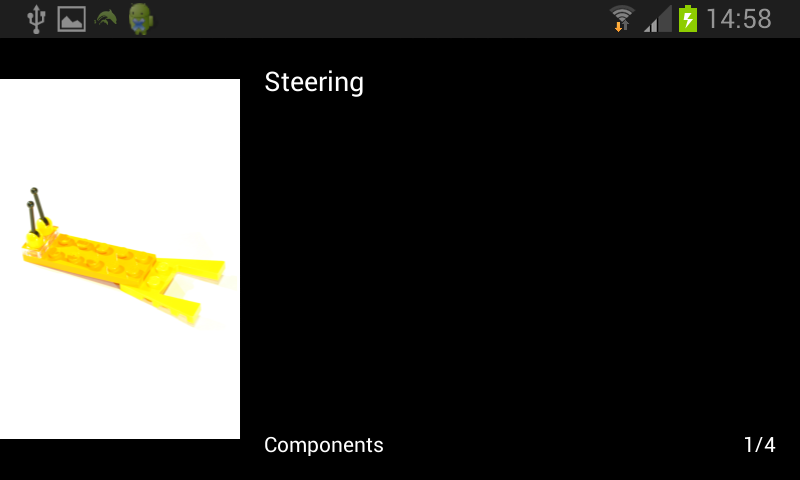
\includegraphics[width=60mm]{images/demoCase/2spL}}}
		\qquad
		\subfloat[The Steering component.]{{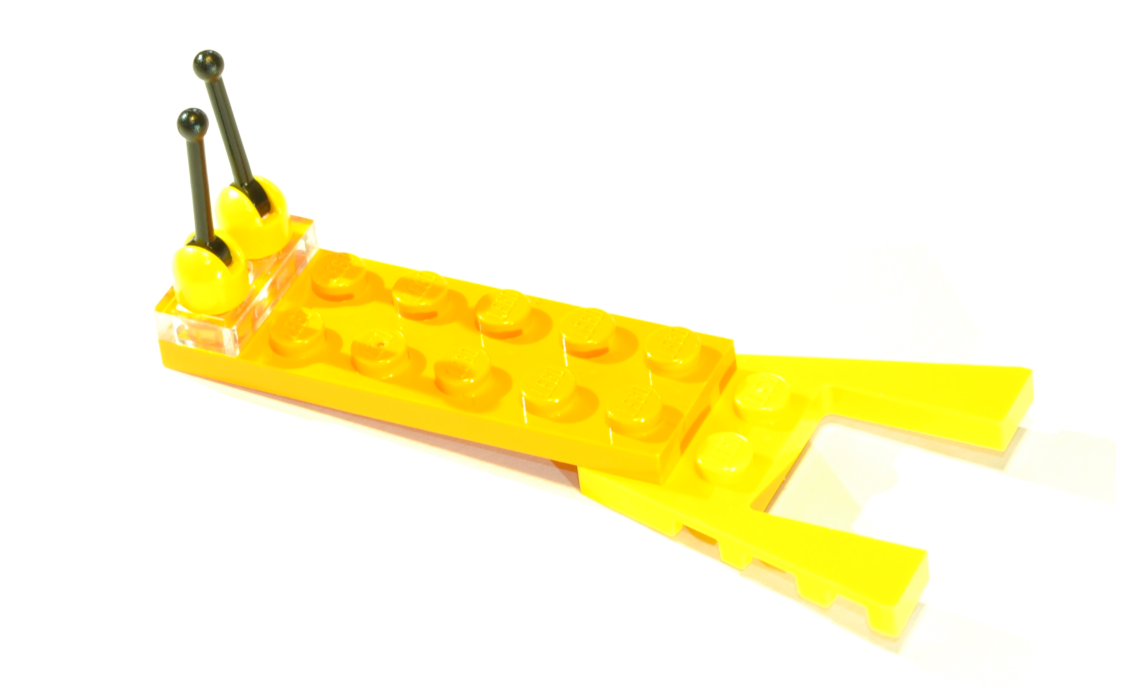
\includegraphics[width=60mm]{images/rawImages/BILD_1}}}
		\caption{The first component.}
		\label{demoCaseSteering}
	\end{figure}

The next slide is the second component slide, seen in Figure~\ref{demoCaseTailLight}, which uses only text to describe the component. The component is called ``Tail Light'', and can be seen in Figure~\ref{demoCaseTailLight}~(c). The reason for not using an image to describe the Tail Light component is since the text was deemed as sufficient enough for the user to distinguish the Tail Light component from the others.

	\begin{figure}[ht!]
		\centering
		\subfloat[The second component card.]{{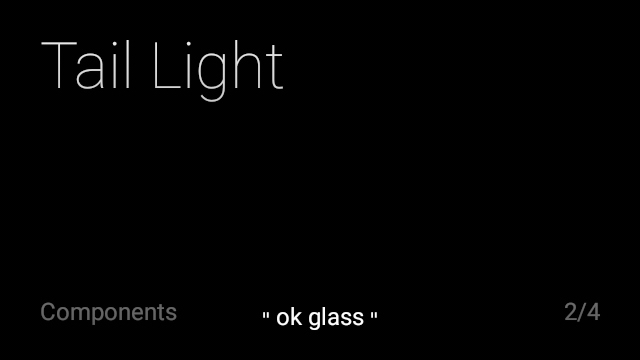
\includegraphics[width=60mm]{images/demoCase/3}}}
		\qquad
		\subfloat[The second component slide.]{{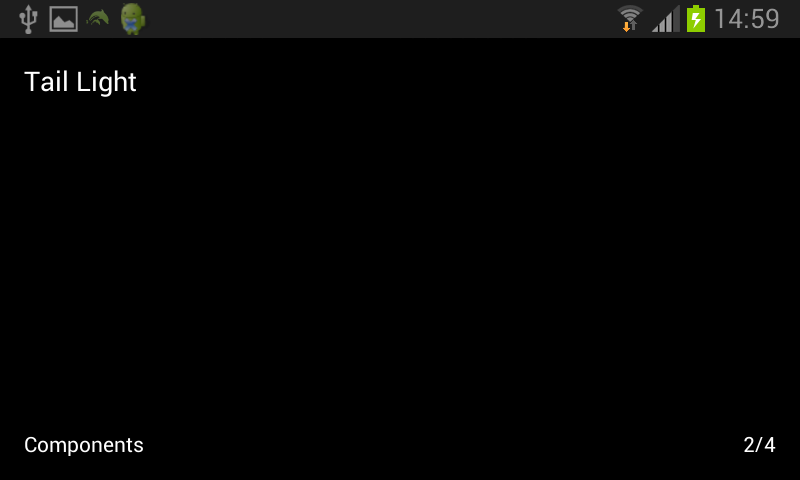
\includegraphics[width=60mm]{images/demoCase/3sp2}}}
		\qquad
		\subfloat[The Tail Light component.]{{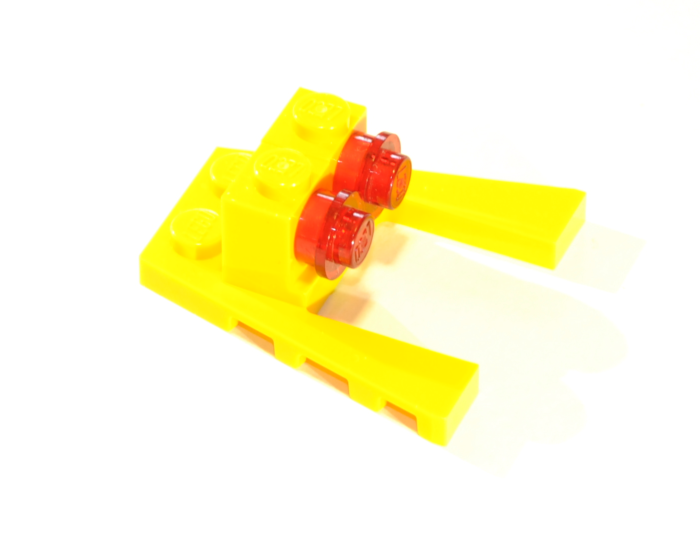
\includegraphics[width=60mm]{images/rawImages/BILD_2}}}
		\caption{The second component.}
		\label{demoCaseTailLight}
	\end{figure}

The fourth slide in the application is the third component slide, seen in Figure~\ref{demoCaseBody}. Similar to the first component slide, the third component slide uses both and image as well as text in order to describe which component the user need. The component is called ``Body'' and can be seen in Figure~\ref{demoCaseBody}~(c). The reason for using both text and an image to describe the Body component is because the component name is a general one and could potentially apply to the Steering component as well.

	\begin{figure}[H]%ht!]
		\centering
		\subfloat[The third component card.]{{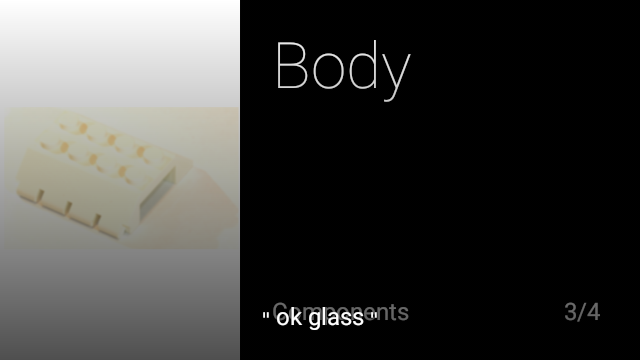
\includegraphics[width=60mm]{images/demoCase/4}}}
		\qquad
		\subfloat[The third component slide.]{{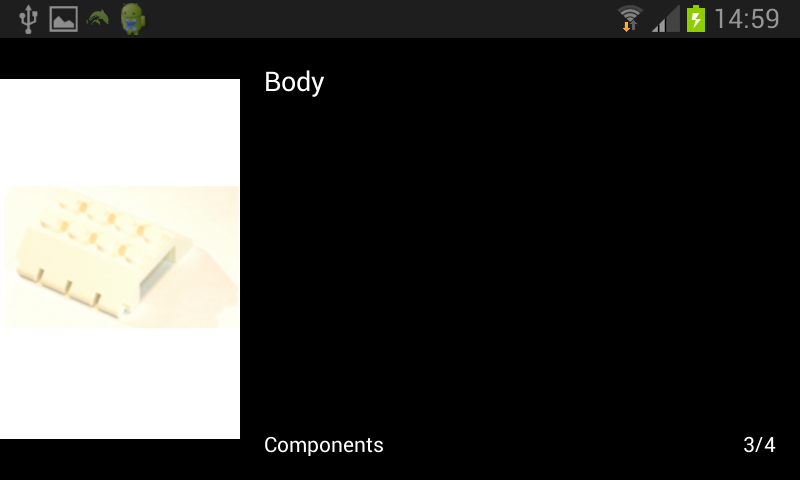
\includegraphics[width=60mm]{images/demoCase/4sp}}}
		\qquad
		\subfloat[The Body component.]{{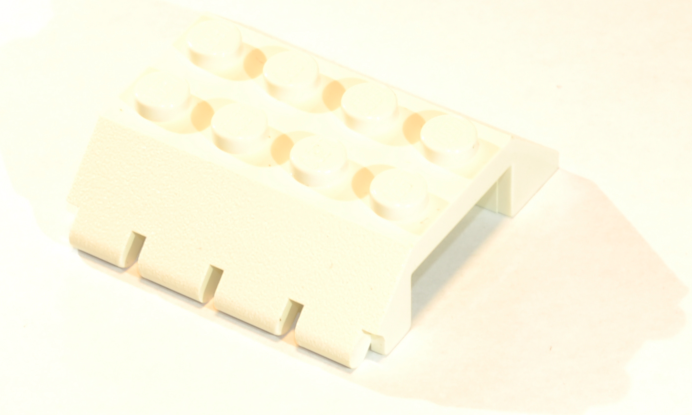
\includegraphics[width=60mm]{images/rawImages/BILD_3}}}
		\caption{The third component.}
		\label{demoCaseBody}
	\end{figure}
	
The next slide is the fourth and last component slide, seen in Figure~\ref{demoCasePirate}. Similar to Figure~\ref{demoCaseTailLight}, the fourth component is also only described in text. The component is called ``Pirate'' and can be seen in Figure~\ref{demoCasePirate}~(c).

	\begin{figure}[H]%ht!]
		\centering
		\subfloat[The fourth component card.]{{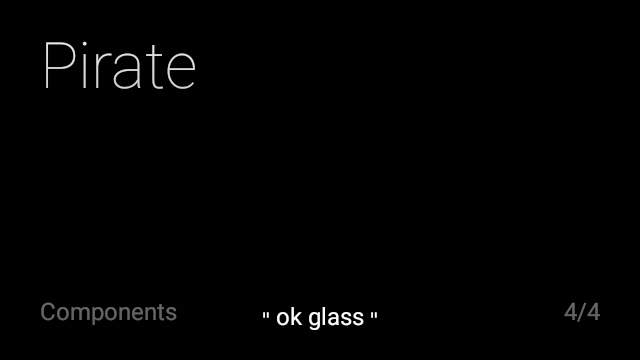
\includegraphics[width=60mm]{images/demoCase/5}}}
		\qquad
		\subfloat[The fourth component slide.]{{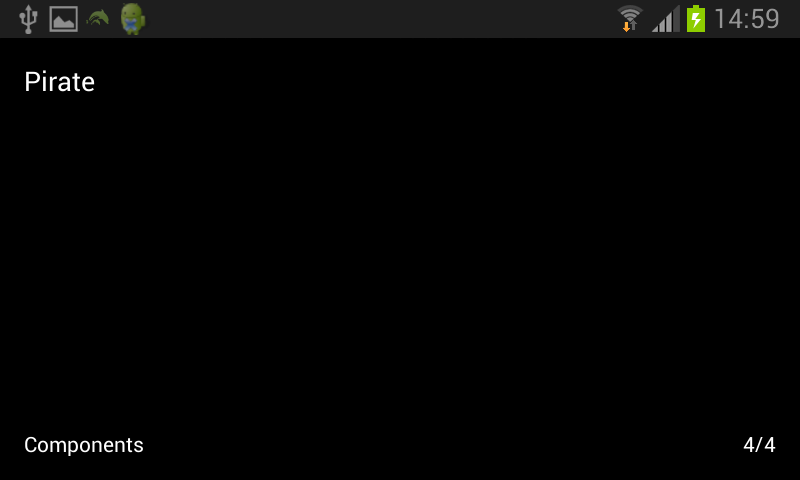
\includegraphics[width=60mm]{images/demoCase/5sp}}}
		\qquad
		\subfloat[The Pirate component.]{{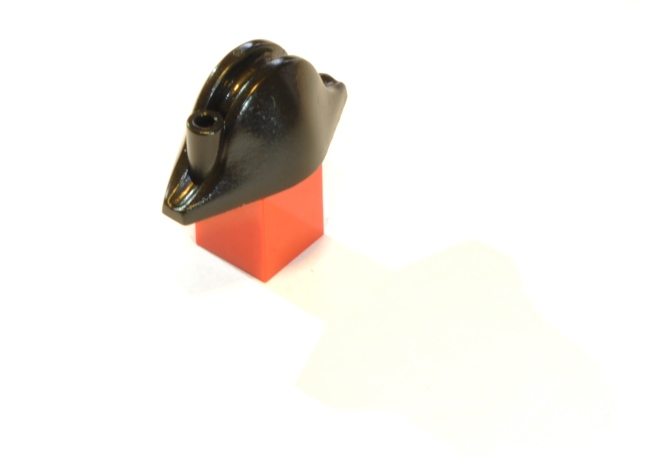
\includegraphics[width=60mm]{images/rawImages/BILD_4}}}
		\caption{The fourth component.}
		\label{demoCasePirate}
	\end{figure}

After the components come the instructions. At this point the user should have gathered all of the components and be ready to assemble the product. The first instruction slide can be seen in Figure~\ref{demoCaseInstruction1}. The goal is to combine the Tail Light component and the Steering component in to what can be seen in Figure~\ref{demoCaseInstruction1}~(c).

	\begin{figure}[H]%ht!]
		\centering
		\subfloat[The first instruction card.]{{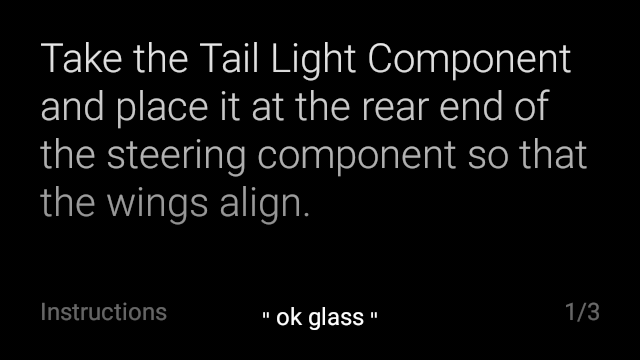
\includegraphics[width=60mm]{images/demoCase/6}}}
		\qquad
		\subfloat[The first instruction slide.]{{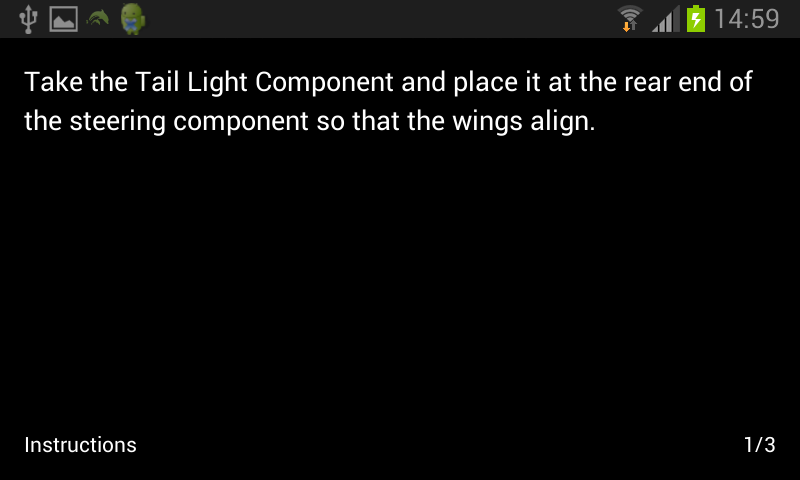
\includegraphics[width=60mm]{images/demoCase/6sp}}}
		\qquad
		\subfloat[The goal of the first instruction.]{{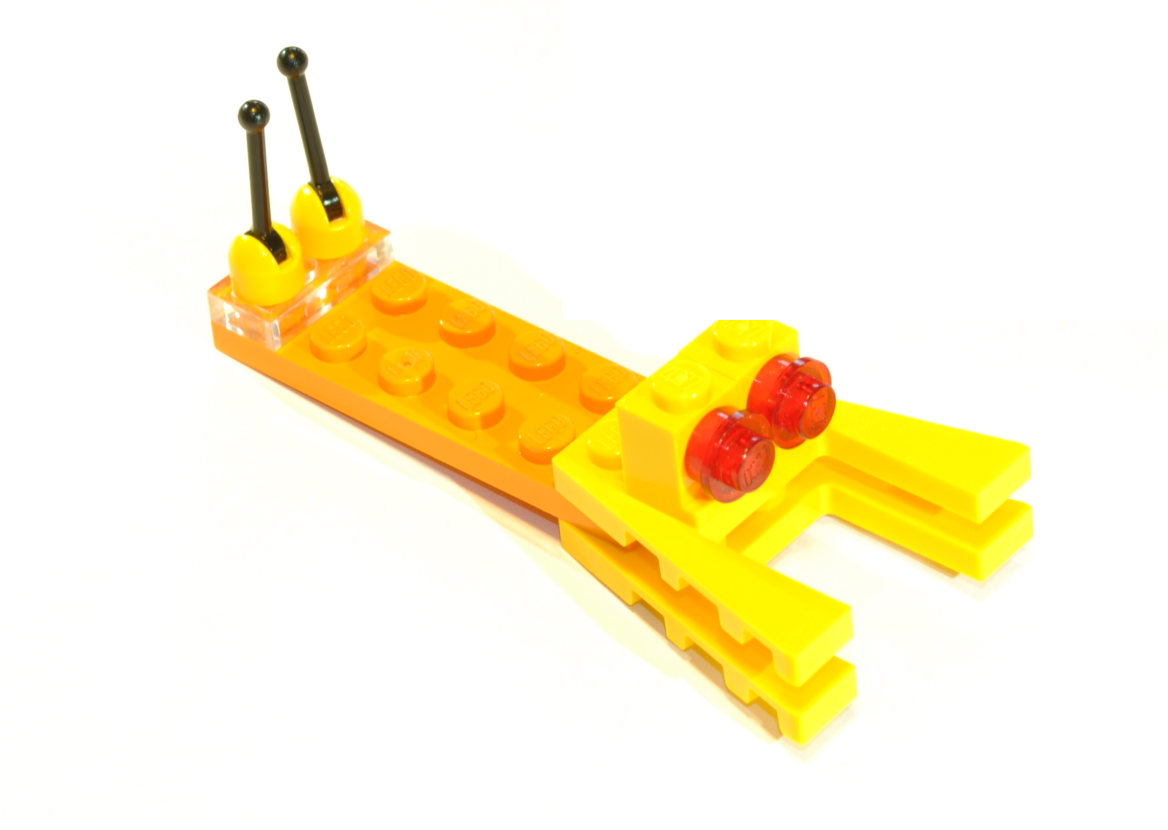
\includegraphics[width=60mm]{images/rawImages/BILD_5}}}
		\caption{The first instruction.}
		\label{demoCaseInstruction1}
	\end{figure}

The second instruction is described with only an image and no text, as seen in Figure~\ref{demoCaseInstruction2}. The reason for this is because the alignment of the components would be difficult to describe in text and a larger image makes it easier for the user to see how the components should fit together. Using both text and an image would mean that the image would be scaled down. The user is with the instruction supposed to combine the Body component and the Pirate component in to what can be seen in Figure~\ref{demoCaseInstruction2}~(c).

	\begin{figure}[H]%ht!]
		\centering
		\subfloat[The second instruction card.]{{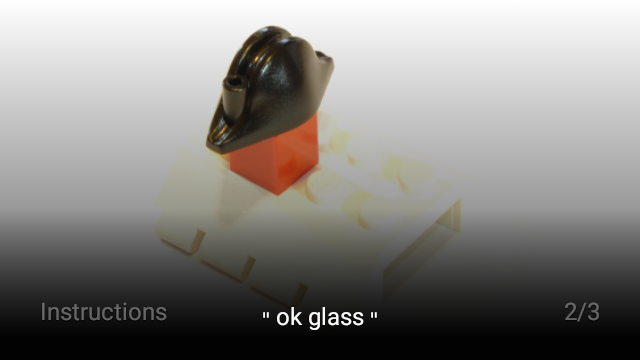
\includegraphics[width=60mm]{images/demoCase/7}}}
		\qquad
		\subfloat[The second instruction slide.]{{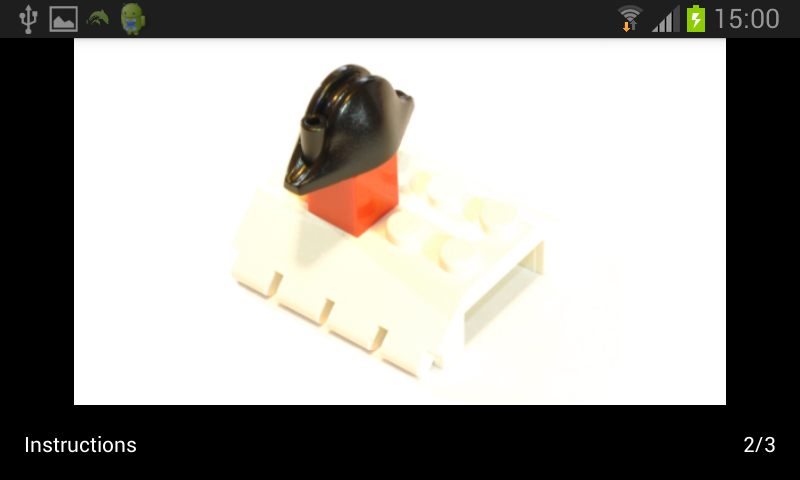
\includegraphics[width=60mm]{images/demoCase/7sp}}}
		\qquad
		\subfloat[The goal of the second instruction.]{{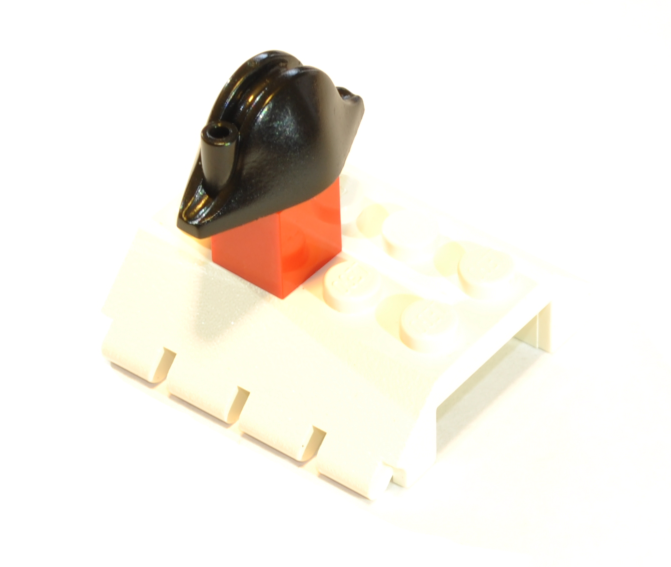
\includegraphics[width=60mm]{images/rawImages/BILD_8}}}
		\caption{The second instruction.}
		\label{demoCaseInstruction2}
	\end{figure}

The final slide, seen in Figure~\ref{demoCaseInstruction3}, describes the final instruction in both text and an image. The reason for using both text and an image is because the text may contain enough information on how to combine the components and the image can be used as visual guideline. Potentially the image could be enough information on its own, and could as such be shown in full scale instead. However, since the image does not need to be full scale it will take up less data space and as such be faster to download compared to a full scale image.

When the user has completed what the third and last instructions say, the product is now fully constructed. As such, the application may now be closed or another QR code may be scanned. In the Google Glass application the user can say ``ok glass'' and then ``Scan again'', in order to bring up the camera and scan another QR code. In the smartphone application the user may press the default back button on the smartphone in order to bring up the camera and scan another QR code.

	\begin{figure}[H]%ht!]
		\centering
		\subfloat[The third instruction card.]{{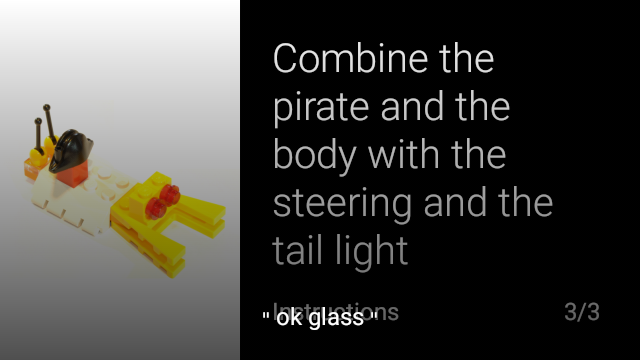
\includegraphics[width=60mm]{images/demoCase/8}}}
		\qquad
		\subfloat[The third instruction slide.]{{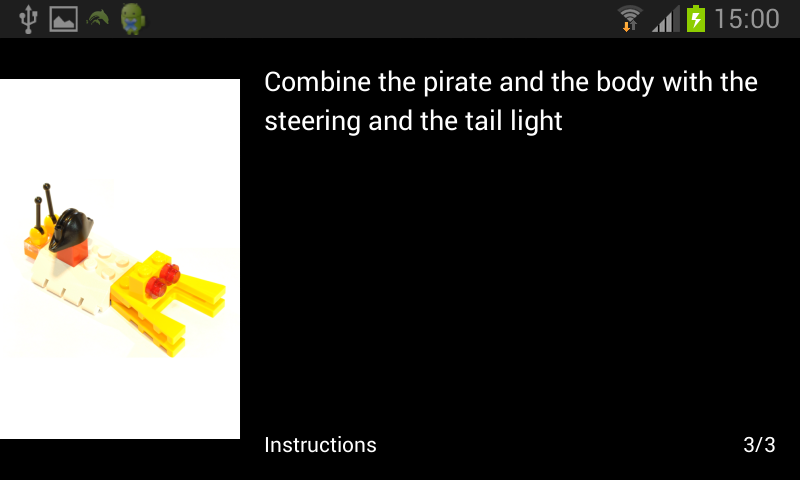
\includegraphics[width=60mm]{images/demoCase/8sp}}}
		\qquad
		\subfloat[The goal of the third instruction.]{{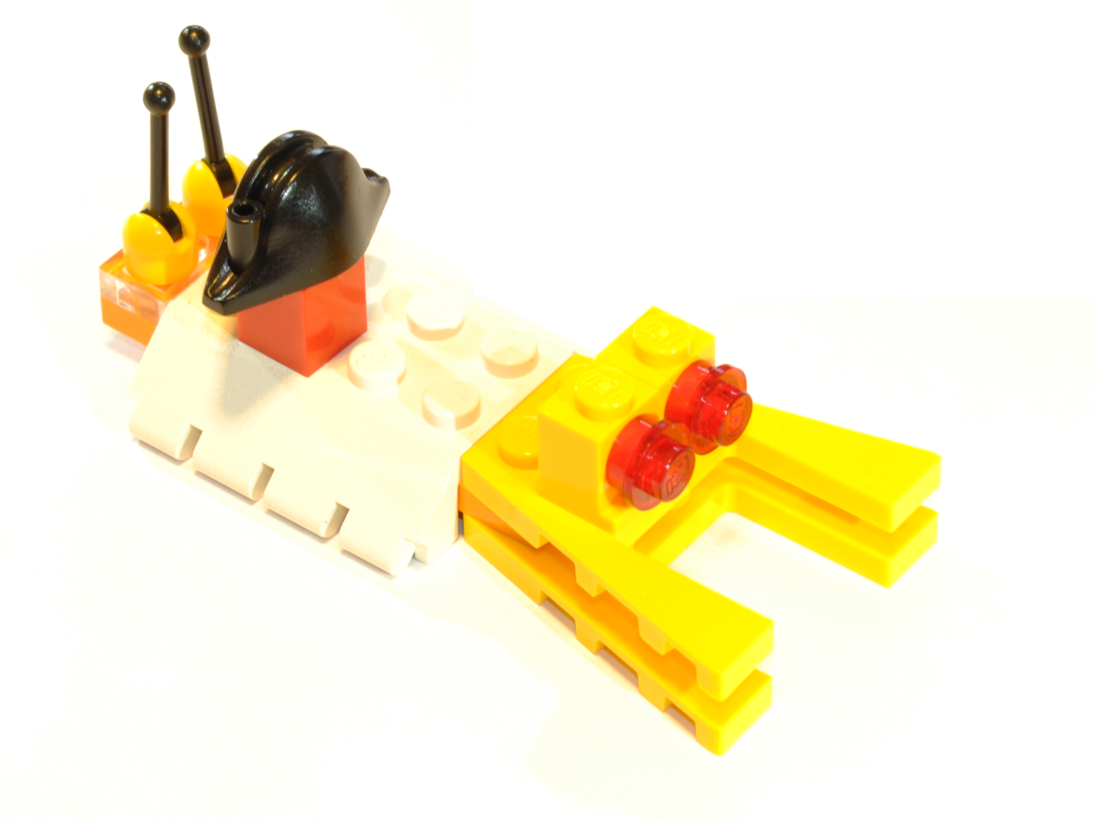
\includegraphics[width=60mm]{images/rawImages/BILD_6}}}
		\caption{The third instruction.}
		\label{demoCaseInstruction3}
	\end{figure}


% done